%%%%%%%%%%%%%%%%%%%%%%%%%%%%%%%%%%%%%%%%%%%%%%%%%%%%%%%%%%%%%%%
\chapter{Resultados}
%\addcontentsline{toc}{chapter}{Resultados} % Añadir a la tabla de contenidos si es que no aparece
\spacing{1.5}

De la consulta 0 obtuve 18,825 resultados, de los cuales podemos ver la cantidad de publicaciones que hay al año y se muestran en la Figura \ref{fig:consulta0} en la cual se puede ver que a partir del 2020 aumentaron drásticamente las publicaciones sobre cienciometría, bibliometría, y los análisis de la literatura. 
\begin{figure}[H]
\centering
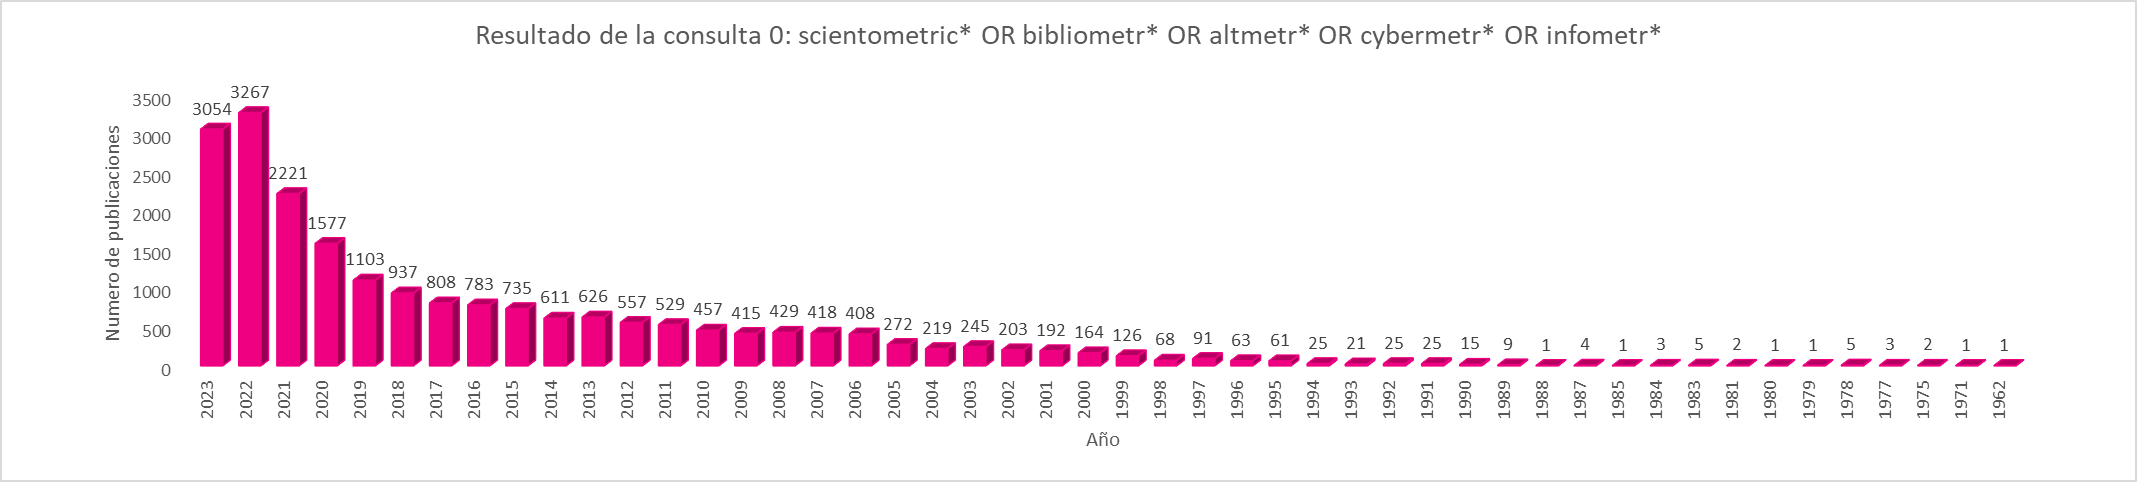
\includegraphics[width=1\textwidth]{Imagenes/consulta0.png}
\caption{\textit{Gráfica de la cantidad de publicaciones por año de la consulta 0}}
\label{fig:consulta0}
\end{figure}
De la consulta 1 obtuve 1,011 resultados de los cuales...\\
De la consulta 2 obtuve 1,784 resultados de los cuales...\\